Hemos hablado de la posibilidad de una pobre calidad de los productos que entreguemos al final de nuestro proyecto. Hemos hablado que es un riesgo potencial y que en principio puede ser evitado o como mínimo prevenido. Durante el desarrollo de la aplicación vamos a asegurar el control de la calidad sometiendo el propio software a un proceso de desarrollo e integración continua. Como hemos mencionado de pasada en la parte de tecnologías, vamos a usar diferentes tecnologías para asegurarnos de que la calidad de nuestra aplicación es la máxima que le podemos ofrecer a nuestro cliente. 

La idea es que nosotros vamos a seguir un proceso de pruebas casi paralelo, aunque siempre un poco retrasado por definición en lo que a pruebas de sistema respecta, ya que probar la funcionalidad de algo, primero tenemos que desarrollarlo. 

Una vez estén implementadas las primeas interfaces de usuario, con sus principales interacciones es cuando se introducirán y diseñarán las principales pruebas de sistema. Además de estas pruebas se desarrollaran, aunque en menor medida pruebas funcionales para los módulos que se considere oportunos y que tengan un comportamiento esperado para una entrada dada. 

Todo este conjunto de pruebas se intentará que queden lo más automatizado posible. Como el objetivo principal es el desarrollo de la aplicación, no se le dará una importancia grande a esta parte, pero si que me gustaría introducir unas cuantas tecnologías de uso diario en el desarrollo ágil de productos software como puede ser Jenkins. Esta tecnología será la principal responsable de la automatización de toda nuestra suite de pruebas. Evidentemente no solo sirve para pruebas, sirve para automatizar procesos de software en general, otro ejemplo que podemos observar es el despliegue de un determinado servicio web en un entorno de desarrollo o producción cuando los cambios necesarios han sido realizados correctamente. 

Podemos ver en la \textbf{Figura \ref{fig:cicd}}, una aproximación del flujo al que se va a someter las diferentes partes de código que desarrollemos en nuestra aplicación.

\vspace{2cm}

\begin{figure}[H]
    \centering
    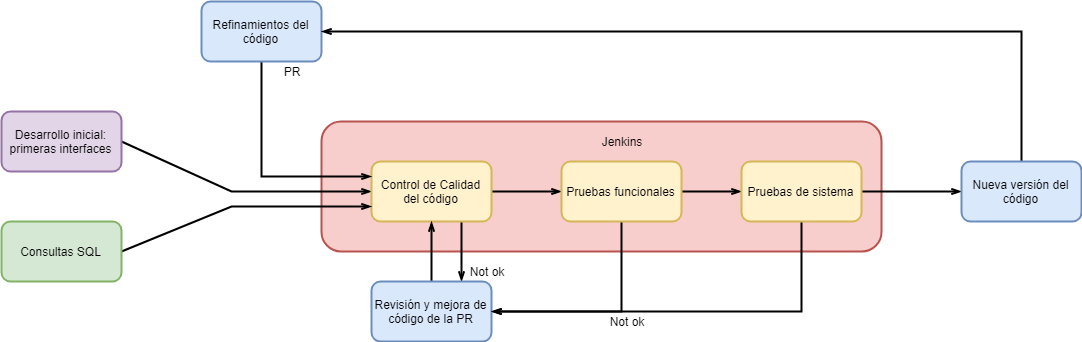
\includegraphics[scale=0.45]{imagenes/planificacionGestion/cicd.png}
    \caption{Flujo de Integración continua}
    \label{fig:cicd}
\end{figure}

\textcolor{red}{diseñar un pequeño diagrama del flujo que seguirán las pruebas y el código de la aplicación}